\documentclass{article}
\usepackage{graphicx,amsmath}
\begin{document}
\title{}
\author{}
\maketitle

Trying to make a smooth time evolution curve.

By looking for a way to fill in spikes and step discontinuities with missing points.

By choosing the best starting order based on which creates the best linear region.

One way to do this might be to do a fit on a segment of the curve, though it is difficult to determine starting and stop points for the fit automatically. It would be possible to iterate over all of them and pick out minimum chisq/dof. just want a line on a semilog plot for some segment of the plot for each value of starting order. The best starting order also has the best chisq/dof. However, it may also be necessary to take the number of DOF into account. Recall that in exact Chi Sq statistics, the expectation value of Chi Sq is not one.


The other way is to look for the most linear set of three points used in the extrapolation. How would you define most linear? smallest residual? smallest relative residual? sum them over three points? Frank and I realized that the three points shoudl identically lie on a line if it is solveable once finf is subtracted; however, it is possible to take the residuals of neighboring points. 

Frank says to check a couple of points first by hand.

Time 472 is one of the discontinuous points for mode $l=2$. I checked all starting order indices by hand, and found several plausible plots and values of finf, summarized in a table and in figures below. The most similar values of finf were for the higher order starting indices. Note that for this case, the lowest starting index lead to an undefined yratio (value of $g(\alpha)$), but that higher starting orders were well defined or even looked really good. For the starting orders that lead to long straight lines, the relative error in finf was on the order of $10^-9$ due to the starting index effect. The best choices seemed to be ones that had a long straight line of several points (4,5,6). These are also the higher modes, which is good, because there is less far to extrapolate to finf. In a sense it is also bad, because it requires more information to extrapolate to finf. This suggests a possible strategy would be to use the fit and the chisq and dof technique. 

\begin{table}
\begin{tabular}{ll}
Starting index & finf\\
2 & 4.18128309016e-05\\
3 & mode failed\\
4 & 4.18128307505e-05\\
5 & 4.18128308245e-05\\
6 & 4.1812830828e-05\\
\end{tabular}
\end{table}


\begin{figure}
  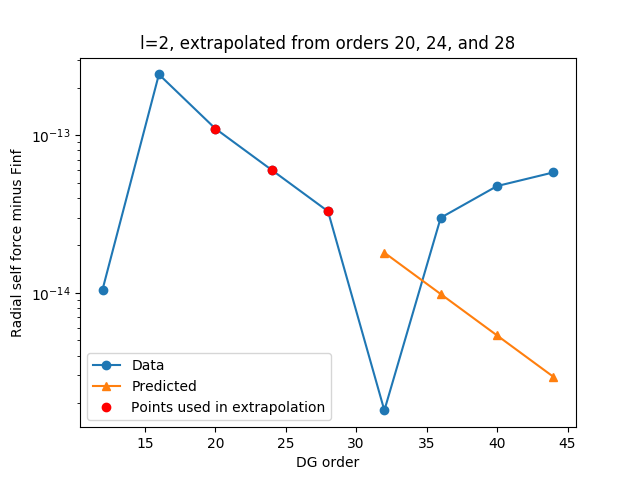
\includegraphics{extrapolate7t472l3i2}
\end{figure}
\begin{figure}
  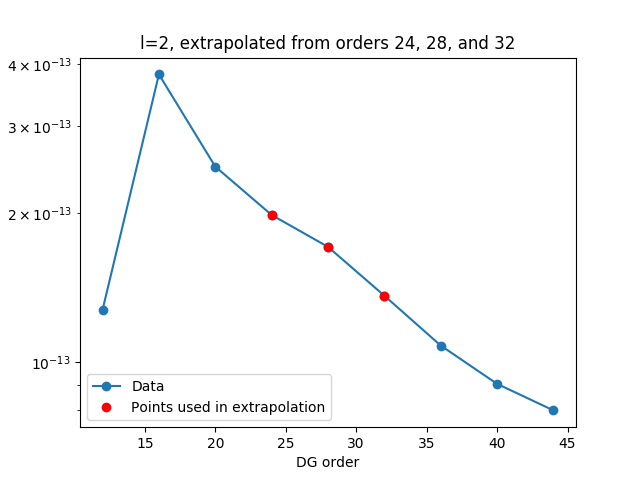
\includegraphics{extrapolate7t472l2i3}
  \caption{Note that the three points used in the extrapolation are not on a line on a semilog scale-- it is not possible to fit an exponential through them. That is why this mode failed.}
\end{figure}
\begin{figure}
  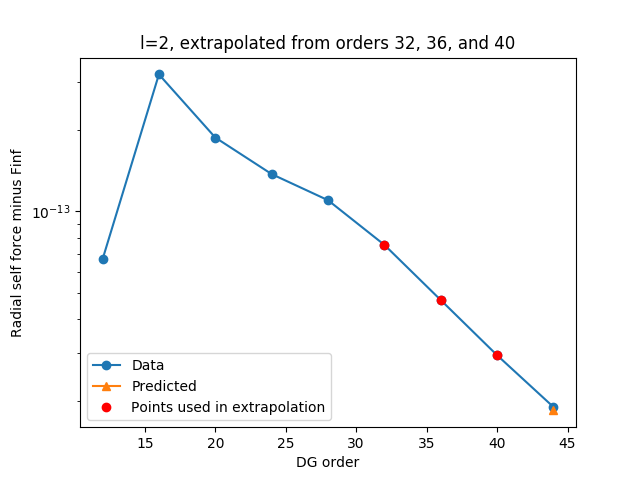
\includegraphics{extrapolate7lt472l2i5}
\end{figure}
\begin{figure}
  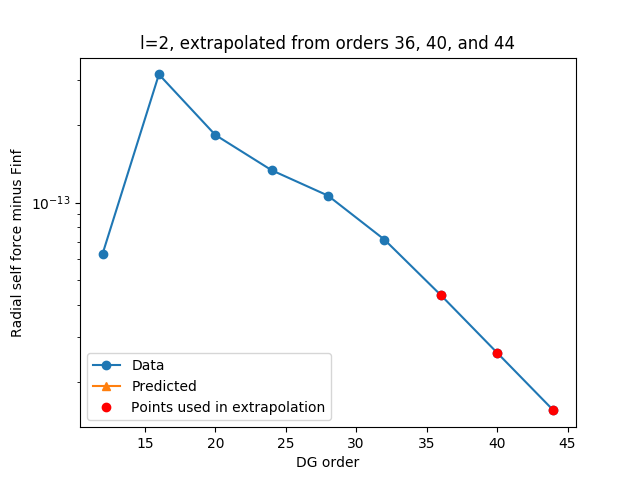
\includegraphics{extrapolate7t472l2i6}
\end{figure}

\begin{figure}
  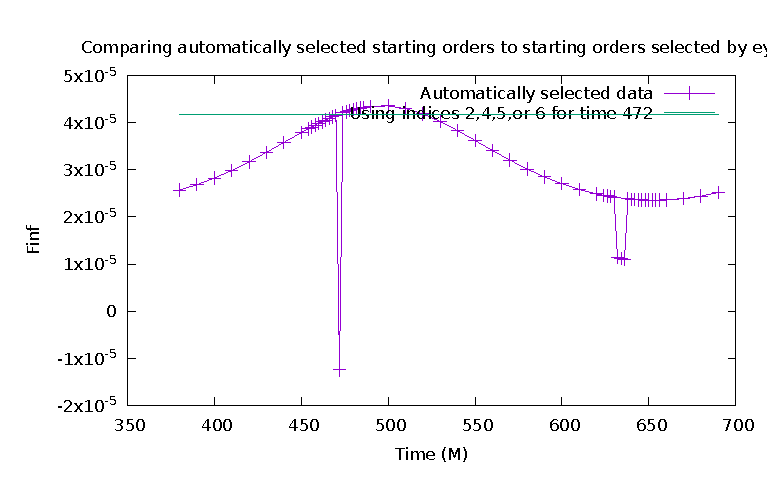
\includegraphics{manuallyChosenBestFinft472}
\end{figure}



\end{document}
